\documentclass{ximera}[font=12pt]

\title{Subtracting Integers: Rule}   % Use xmlatex all -s to compile when SERVE refuses to work.
\author{Kelly Stady}
\license{CC: 0}         % replace with an appropriate license, or set it in xmPreamble

\begin{document}

\begin{abstract}

\end{abstract}

\maketitle
\label{xim:SubtractIntIntroActivity}

\section*{Rule for Subtracting Integers}

Our work with elevation spans demonstrated that \textbf{subtracting a number is equivalent to adding its opposite}. This rule is stated formally below.

\begin{procedure}[\textbf{Subtracting Integers}]


If $a$ and $b$ are integers, then $a-b = a + (-b).$  \\


\textbf{Examples} \ Subtracting a number is equivalent to adding its opposite. \\ 


$-1 - (-12) = -1 + 12$ \\

$-1 - 12 = -1 + (-12)$


\end{procedure}

\textbf{Remarks:}

\begin{enumerate}

\item Once the subtraction problem has been rewritten as addition, use the rules for adding integers to find the answer.

\item When you subtract a positive number from a \emph{larger} positive number, there is no reason to rewrite the subtraction problem as
addition of the opposite.  For example, you don't need to rewrite $7-2$ as $7 + (-2)$ to figure out that the answer is 5.  So, \textbf{only rewrite subtraction as addition
if you need to}.
\end{enumerate}


\begin{problem}
Rewrite the subtraction problem as an equivalent addition problem.  Then find the answer.

\[ -6 - (-3) \]

\begin{multipleChoice}
\choice{$-6 - (-3) = 6 + 3$}
\choice{$-6 - (-3) = -6 + (-3)$}
\choice[correct]{$-6 - (-3) = -6 + 3$}
\choice{$-6 - (-3) = 6 + (-3)$}
\end{multipleChoice}

\begin{problem}
Answer  $ = \answer{-3}$

\end{problem}
\end{problem}


%VIDEO!!!!!!!!!!!!!!!!!!!!!!!


\begin{problem}
Rewrite the subtraction problem as an equivalent addition problem.  Then find the answer.

\[ -2 - 10 \]

\begin{multipleChoice}
\choice{$-2 - 10 = 2 + (-10)$}
\choice{$-2 - 10 = 2 + 10$}
\choice{$-2 - 10 = -2 + 10$}
\choice[correct]{$-2 - 10 = -2 + (-10)$}
\end{multipleChoice}

\begin{problem}
Answer $ = \answer{-12}$

\end{problem}
\end{problem}


\begin{problem}
How many degrees warmer is $100^\circ$F than $-80^\circ$F?

Write the subtraction problem to find the answer.

\begin{multipleChoice}
\choice{$100 - 80$}
\choice[correct]{$100 - (-80)$}
\choice{$-100 - 80$}
\choice{$-100 - (-80)$}
\end{multipleChoice}

\begin{problem}
Write the subtraction problem as an equivalent addition problem.  Then find the answer. 

~ \\[0.5em]

\begin{multipleChoice}
\choice{$100 - (-80) = 100 + (-80)$}
\choice{$100 - (-80) = -100 + 80 $}
\choice{$100 - (-80) = -100 + (-80)$}
\choice[correct]{$100 - (-80) = 100 + 80$}
\end{multipleChoice}

~ \\[0.5em]

Answer $= \begin{prompt} \answer{180} \end{prompt}$ degrees


\begin{center}
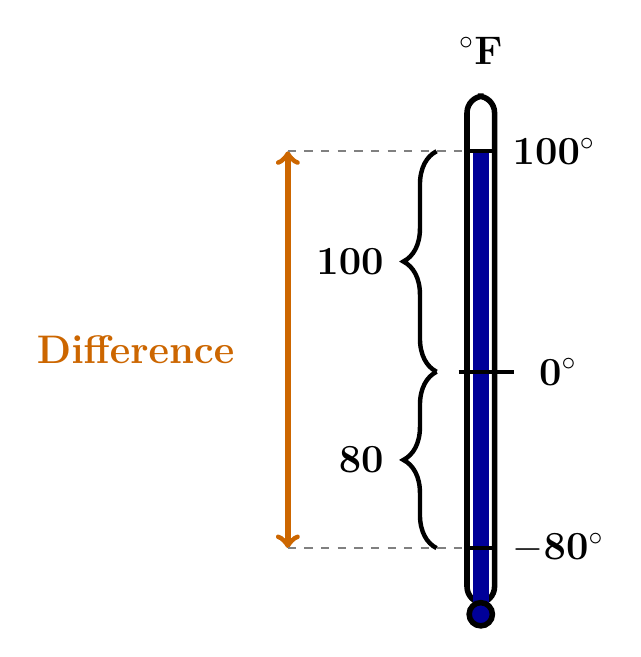
\begin{tikzpicture}[scale = 0.7, y=0.4mm, x=1mm]
    % --- THERMOMETER BODY ---
    % Outer Tube
    \draw[line width=2pt, black, fill=white, rounded corners=6pt] (-2.5,-105) rectangle (2.5,125);

    % Inner Blue Liquid (up to 100) for Accessibility
    \fill[blue!60!black] (-1.5,-105) -- (-1.5,100) -- (1.5,100) -- (1.5,-105) -- cycle;

    % Bulb at the bottom
    \filldraw[blue!60!black, draw=black, line width=2pt] (0,-110) circle (6pt);

    % --- VERTICAL AXIS (Labels and Units) ---
    \node[above=8pt] at (0,125) {\Large\textnormal{$^\circ$\textbf{F}}};

    % --- ZERO POINT  ---
    \draw[black, ultra thick] (-4,0) -- (6,0)
        node[right, xshift=5pt] {\Large\textnormal{\textbf{0$^\circ$}}};

    % --- KEY POINTS ---
    % 100 Degrees
    \draw[ultra thick] (-3,100) -- (3,100);
    \node[right, xshift=8pt] at (0,100) {\Large\textnormal{\textbf{100}$^\circ$}};

    % -80 Degrees
    \draw[ultra thick] (-3,-80) -- (3,-80);
    \node[right, xshift=8pt] at (0,-80) {\Large\textbf{\textnormal{$-$\textbf{80}$^\circ$}}};

    % --- BRACES ---
    \draw [decorate, decoration={brace, amplitude=12pt, raise=10pt}, ultra thick] (-3,-80) -- (-3,0)
        node [midway, left=25pt] {\Large\textnormal{\textbf{80}}};

    \draw [decorate, decoration={brace, amplitude=12pt, raise=10pt}, ultra thick] (-3,0) -- (-3,100)
        node [midway, left=25pt] {\Large \textnormal{\textbf{100}}};

    % --- TOTAL DISTANCE ARROW ---
    \draw[<->, orange!80!black, line width=2pt] (-35,-80) -- (-35,100)
        node[midway, left=15pt, align=center] {\textnormal{\Large \textbf{Difference}}};

    % --- DASHED GUIDES ---
    \draw[dashed, gray, thick] (-35,100) -- (-3,100);
    \draw[dashed, gray, thick] (-35,-80) -- (-3,-80);

\end{tikzpicture}
\end{center}


\end{problem}
\end{problem}

\subsection*{Subtracting a Negative Number}

You may have noticed that \textbf{subtracting a negative} number is equivalent to \textbf{adding a positive} number.  This becomes intuitive when we think in terms of money.  Imagine your checking account balance is \$900 and the bank realizes that they accidently charged you a \$30 $(-30)$ overdraft fee last month.  Once the bank removes (subtracts) the overdraft fee, your net balance increases.
\begin{eqnarray*}
900-(-30) &=& 900 + 30 \\
          &=& 930
\end{eqnarray*}
Removing a debt is the same as gaining a profit.

\end{document}